\chapter{Experiments}
\label{ch:experiments}

\section{Experimental Setup}
\label{sec:setup}

The experiments evaluate whether diffusion-based heatmap solvers can be trained and
fine-tuned for increasingly constrained routing problems. TSP is used as the baseline setting,
CVRP tests whether the approach remains useful under vehicle-capacity constraints, and MDVRP
tests an initial multi-depot assignment extension.

Two compute environments were used. TSP supervised and CADO experiments were run locally on
an Apple M4 Pro machine with 24 GB unified memory using the PyTorch MPS backend. Larger CVRP
and MDVRP supervised runs were executed remotely on a VESSL A100 instance. All main runs use
seed 42. Supervised training uses AdamW with learning rate $2\times10^{-4}$, weight decay
$10^{-4}$, cosine learning-rate decay, and gradient clipping at norm 1.0. CADO fine-tuning
uses AdamW with learning rate $10^{-4}$, no weight decay, LoRA rank 2, one selectively
fine-tuned final layer, and $M_{\mathrm{train}}=5$. The CADO evaluation step count follows the
individual experiment configuration.

\section{Datasets}
\label{sec:datasets}

The datasets consist of synthetic Euclidean routing instances with solver-generated labels.
TSP-50 contains 128,000 instances solved by Concorde. CVRP-50 contains single-depot instances
with 50 customers generated from the X-style distribution and solved by PyVRP. The CVRP file
used by the main run contains 128,000 labeled instances. The main MDVRP run uses a generated
dataset of 64,000 multi-depot instances with 50 customers.

For supervised training, the dataset is split into 90\% training and 10\% validation. To keep
validation cost manageable, each validation pass evaluates a fixed subset: 500 instances for
the supervised TSP, CVRP, and MDVRP runs, 100 instances for the short TSP CADO pilot, 200
instances for the extended TSP CADO run, and 100 instances for CVRP CADO.

\section{Baselines and Metrics}
\label{sec:metrics}

The primary baseline is the supervised DIFUSCO checkpoint trained with cross-entropy on
solver-generated labels. CADO fine-tuning is evaluated as a second-stage improvement over that
checkpoint. For TSP and CVRP, the main metric is optimality gap:
\[
\mathrm{Gap}(\%) =
\frac{L_{\mathrm{pred}} - L_{\mathrm{gt}}}{L_{\mathrm{gt}}}\times 100.
\]
The decoded length $L_{\mathrm{pred}}$ is measured after greedy decoding and 2-opt
post-processing. For CVRP, the validation also reports the capacity-violation rate. For MDVRP,
the current implementation reports depot assignment accuracy and capacity-violation rate,
because full route-cost evaluation for MDVRP is not yet integrated into the training loop.

\section{Main Results}
\label{sec:main-results}

\begin{table}[t]
\centering
\caption{Summary of main experimental results. Lower gap is better; higher MDVRP assignment
accuracy is better.}
\label{tab:main-results}
\begin{tabular}{llrrl}
\toprule
Problem & Method & Best metric & Final metric & Notes \\
\midrule
TSP-50 & DIFUSCO SL & 4.46\% gap & 4.46\% gap & small model \\
TSP-50 & CADO, 100 epochs & 3.77\% gap & 3.77\% gap & SR, eval subset 100 \\
TSP-50 & CADO, 1000 epochs & 3.96\% gap & 4.03\% gap & SR, eval subset 200 \\
CVRP-50 & DIFUSCO SL & 25.96\% gap & 35.51\% gap & paper model, 2-opt \\
CVRP-50 & CADO, 1000 epochs & 20.24\% gap & 47.16\% gap & best at epoch 470 \\
MDVRP-50 & DIFUSCO SL & 81.89\% acc. & 55.75\% acc. & assignment only \\
\bottomrule
\end{tabular}
\end{table}

The TSP results show that CADO fine-tuning can improve a supervised diffusion solver even with
a small model. The supervised TSP-50 baseline reaches a 4.46\% validation gap. A 100-epoch
CADO run improves this to 3.77\%, a 0.69 percentage-point absolute reduction and a 15.4\%
relative reduction in gap. Extending the run to 1000 epochs gives a best gap of 3.96\%, with a
final gap of 4.03\%. Because the extended run uses a larger validation subset than the
100-epoch pilot, the two CADO numbers should not be compared point-by-point; both indicate
that RL fine-tuning improves over the supervised starting point, but the gains are modest and
noisy.

\begin{figure}[t]
\centering
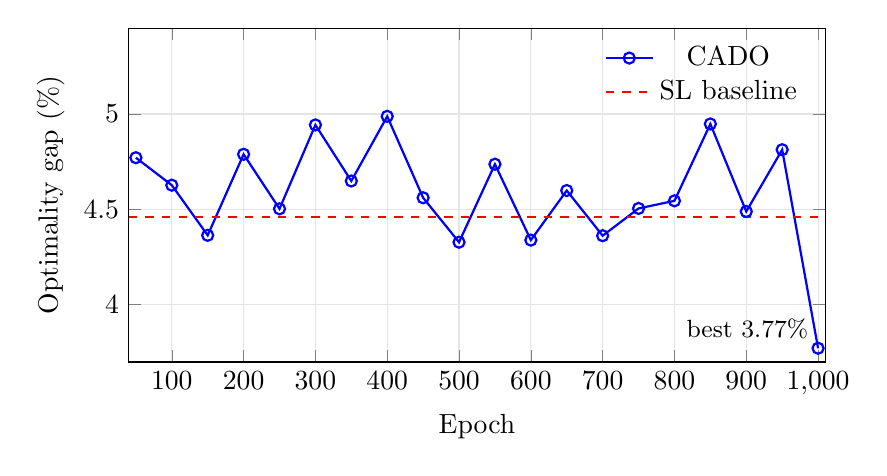
\begin{tikzpicture}
\begin{axis}[
  width=0.86\textwidth,
  height=0.48\textwidth,
  xlabel={Epoch},
  ylabel={Optimality gap (\%)},
  xmin=40,
  xmax=1010,
  ymin=3.7,
  ymax=5.45,
  grid=both,
  grid style={draw=gray!20},
  legend style={draw=none, fill=none, at={(0.98,0.98)}, anchor=north east},
]
\addplot+[mark=o, thick] coordinates {
  (50,4.771) (100,4.627) (150,4.364) (200,4.789)
  (250,4.503) (300,4.943) (350,4.649) (400,4.988)
  (450,4.561) (500,4.328) (550,4.737) (600,4.339)
  (650,4.599) (700,4.362) (750,4.505) (800,4.545)
  (850,4.948) (900,4.489) (950,4.813) (1000,3.772)
};
\addlegendentry{CADO}

\addplot+[mark=none, dashed, thick] coordinates {
  (40,4.46) (1010,4.46)
};
\addlegendentry{SL baseline}

\node[anchor=south east, font=\small] at (axis cs:1000,3.772) {best 3.77\%};
\end{axis}
\end{tikzpicture}

\caption{TSP-50 validation gap during the extended CADO run. The dashed line shows the
supervised checkpoint used to initialize fine-tuning.}
\label{fig:tsp-cado-gap}
\end{figure}

The CVRP results are more challenging. The supervised CVRP-50 run with the paper-size model
and per-route 2-opt reaches a best validation gap of 25.96\% at epoch 10, but the final epoch
degrades to 35.51\%. CADO fine-tuning improves the best checkpoint to 20.24\% at epoch 470,
showing that cost-aware fine-tuning can improve decoded CVRP quality. However, the same run
collapses later, ending at 47.16\% gap. Thus, for CVRP the useful result is the best
validation-selected checkpoint, not the final checkpoint.

\begin{figure}[t]
\centering
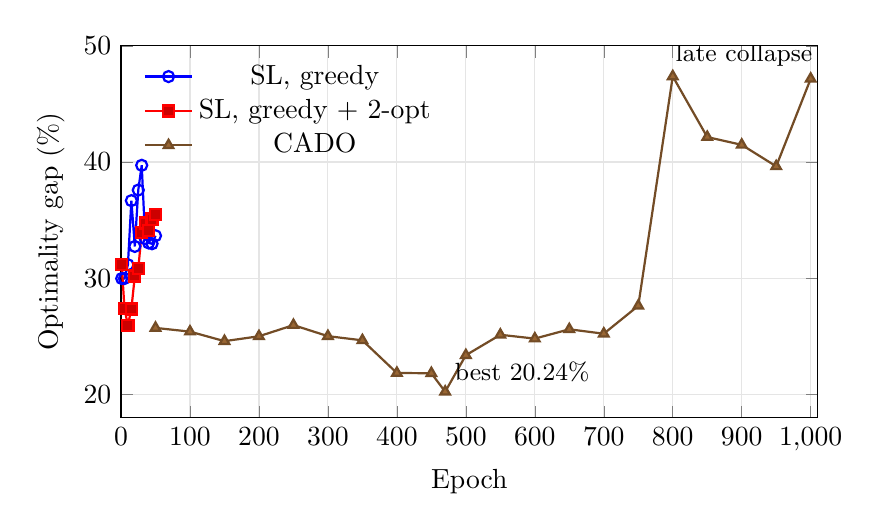
\begin{tikzpicture}
\begin{axis}[
  width=0.86\textwidth,
  height=0.52\textwidth,
  xlabel={Epoch},
  ylabel={Optimality gap (\%)},
  xmin=0,
  xmax=1010,
  ymin=18,
  ymax=50,
  grid=both,
  grid style={draw=gray!20},
  legend style={draw=none, fill=none, at={(0.02,0.98)}, anchor=north west},
]
\addplot+[mark=o, thick] coordinates {
  (1,29.98) (5,29.98) (10,31.17) (15,36.68)
  (20,32.74) (25,37.59) (30,39.72) (35,33.41)
  (40,33.04) (45,32.97) (50,33.66)
};
\addlegendentry{SL, greedy}

\addplot+[mark=square*, thick] coordinates {
  (1,31.20) (5,27.39) (10,25.96) (15,27.36)
  (20,30.19) (25,30.82) (30,33.92) (35,34.75)
  (40,34.12) (45,35.09) (50,35.51)
};
\addlegendentry{SL, greedy + 2-opt}

\addplot+[mark=triangle*, thick] coordinates {
  (50,25.73) (100,25.41) (150,24.59) (200,25.01)
  (250,25.97) (300,25.02) (350,24.66) (400,21.85)
  (450,21.83) (470,20.24) (500,23.38) (550,25.14)
  (600,24.81) (650,25.61) (700,25.23) (750,27.63)
  (800,47.37) (850,42.15) (900,41.48) (950,39.63)
  (1000,47.16)
};
\addlegendentry{CADO}

\node[anchor=south west, font=\small] at (axis cs:470,20.24) {best 20.24\%};
\node[anchor=south west, font=\small] at (axis cs:790,47.37) {late collapse};
\end{axis}
\end{tikzpicture}

\caption{CVRP-50 validation gap for supervised decoding variants and CADO fine-tuning. 2-opt
improves the best supervised checkpoint, while CADO reaches a lower best gap but later
collapses.}
\label{fig:cvrp-validation-gap}
\end{figure}

The MDVRP experiment is best interpreted as an implementation and diagnostic result rather
than a full routing benchmark. The supervised assignment model reaches 81.89\% assignment
accuracy at the first validation point, while the final model drops to 55.75\%. Capacity
violations remain at 0\% throughout validation. This indicates that the current assignment
decoder preserves aggregate capacity but that the supervised diffusion objective does not
maintain alignment with depot assignment accuracy over continued training.

\begin{figure}[t]
\centering
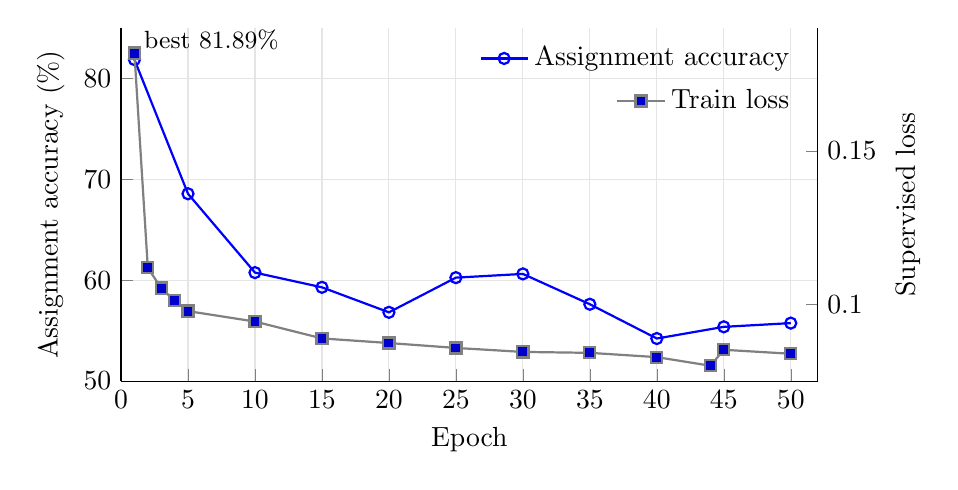
\begin{tikzpicture}
\begin{axis}[
  width=0.86\textwidth,
  height=0.50\textwidth,
  xlabel={Epoch},
  ylabel={Assignment accuracy (\%)},
  xmin=0,
  xmax=52,
  ymin=50,
  ymax=85,
  grid=both,
  grid style={draw=gray!20},
  axis y line*=left,
  axis x line*=bottom,
  legend style={draw=none, fill=none, at={(0.98,0.98)}, anchor=north east},
]
\addplot+[mark=o, thick] coordinates {
  (1,81.89) (5,68.58) (10,60.76) (15,59.30)
  (20,56.82) (25,60.26) (30,60.63) (35,57.62)
  (40,54.22) (45,55.38) (50,55.75)
};
\addlegendentry{Assignment accuracy}
\node[anchor=south west, font=\small] at (axis cs:1,81.89) {best 81.89\%};
\end{axis}

\begin{axis}[
  width=0.86\textwidth,
  height=0.50\textwidth,
  xmin=0,
  xmax=52,
  ymin=0.075,
  ymax=0.19,
  axis y line*=right,
  axis x line=none,
  ylabel={Supervised loss},
  legend style={draw=none, fill=none, at={(0.98,0.86)}, anchor=north east},
]
\addplot+[mark=square*, thick, gray] coordinates {
  (1,0.1819) (2,0.1119) (3,0.1053) (4,0.1012)
  (5,0.0978) (10,0.0944) (15,0.0889) (20,0.0874)
  (25,0.0858) (30,0.0845) (35,0.0842) (40,0.0828)
  (44,0.0800) (45,0.0852) (50,0.0839)
};
\addlegendentry{Train loss}
\end{axis}
\end{tikzpicture}

\caption{MDVRP-50 assignment accuracy and supervised loss. The loss decreases steadily, but
assignment accuracy degrades after the first validation point.}
\label{fig:mdvrp-assignment-accuracy}
\end{figure}

\section{Ablations}
\label{sec:ablations}

Several implementation-level ablations and comparisons were informative.

\paragraph{Effect of 2-opt on CVRP.}
The CVRP supervised baseline was evaluated with and without per-route 2-opt. Greedy decoding
alone reached approximately 29.98\% best validation gap, while enabling 2-opt improved the
best gap to 25.96\%. This confirms that local refinement is an important part of the
heatmap-to-route pipeline for CVRP.

\paragraph{Reward mode.}
Early TSP CADO pilots showed that LCR was ineffective with the weak supervised baseline used
in this thesis: the reward produced little usable relative signal. Switching to SR with
batch-normalized advantages and learning rate $10^{-4}$ produced measurable improvements. For
CVRP, the main CADO configuration uses LCR, but the run still exhibits strong instability,
suggesting that reward scaling and checkpoint selection remain central issues.

\paragraph{Training duration.}
Longer CADO training is not uniformly beneficial. On TSP, the 1000-epoch run improves the
average validation band only slowly and remains noisy. On CVRP, the 1000-epoch run improves
until the middle of training and then collapses. These results support validation-based early
stopping rather than selecting the final checkpoint by default.

\paragraph{Parameter-efficient fine-tuning.}
Hybrid-FT substantially reduces the number of trainable parameters. In the TSP small-model
run, only 178K of 953K parameters are trainable. This makes local RL fine-tuning practical,
but the very small gradient norms and nearly flat mean log-probabilities observed in the TSP
runs suggest limited exploration.

\section{Discussion}
\label{sec:discussion}

The experiments support three conclusions. First, the heatmap-plus-decoder design can produce
feasible routing solutions, and CADO-style fine-tuning can improve the best decoded solution
quality over supervised training. This is clearest on TSP and also visible in CVRP at the best
checkpoint.

Second, supervised denoising loss is not a reliable proxy for decoded routing quality. In both
CVRP and MDVRP, training loss continues to decrease while validation gap or assignment
accuracy worsens. This empirically matches the objective-mismatch argument motivating CADO:
the network can become better at predicting labels without becoming better after the
non-differentiable decoder.

Third, CADO fine-tuning introduces its own stability challenges. The CVRP CADO run improves
substantially at epoch 470 but collapses by epoch 1000. The TSP runs show smaller but noisy
improvements. Therefore, the current implementation should be viewed as a successful
proof-of-concept for cost-aware fine-tuning rather than a final state-of-the-art solver.
Future experiments need larger validation subsets, early stopping, stronger exploration
regularization, and full MDVRP route-cost evaluation.
